\documentclass[]{book}
\usepackage{lmodern}
\usepackage{amssymb,amsmath}
\usepackage{ifxetex,ifluatex}
\usepackage{fixltx2e} % provides \textsubscript
\ifnum 0\ifxetex 1\fi\ifluatex 1\fi=0 % if pdftex
  \usepackage[T1]{fontenc}
  \usepackage[utf8]{inputenc}
\else % if luatex or xelatex
  \ifxetex
    \usepackage{mathspec}
  \else
    \usepackage{fontspec}
  \fi
  \defaultfontfeatures{Ligatures=TeX,Scale=MatchLowercase}
\fi
% use upquote if available, for straight quotes in verbatim environments
\IfFileExists{upquote.sty}{\usepackage{upquote}}{}
% use microtype if available
\IfFileExists{microtype.sty}{%
\usepackage{microtype}
\UseMicrotypeSet[protrusion]{basicmath} % disable protrusion for tt fonts
}{}
\usepackage[margin=1in]{geometry}
\usepackage{hyperref}
\hypersetup{unicode=true,
            pdftitle={Text Analysis with R},
            pdfauthor={Claudia Engel, Scott Bailey},
            pdfborder={0 0 0},
            breaklinks=true}
\urlstyle{same}  % don't use monospace font for urls
\usepackage{natbib}
\bibliographystyle{apalike}
\usepackage{color}
\usepackage{fancyvrb}
\newcommand{\VerbBar}{|}
\newcommand{\VERB}{\Verb[commandchars=\\\{\}]}
\DefineVerbatimEnvironment{Highlighting}{Verbatim}{commandchars=\\\{\}}
% Add ',fontsize=\small' for more characters per line
\usepackage{framed}
\definecolor{shadecolor}{RGB}{248,248,248}
\newenvironment{Shaded}{\begin{snugshade}}{\end{snugshade}}
\newcommand{\AlertTok}[1]{\textcolor[rgb]{0.94,0.16,0.16}{#1}}
\newcommand{\AnnotationTok}[1]{\textcolor[rgb]{0.56,0.35,0.01}{\textbf{\textit{#1}}}}
\newcommand{\AttributeTok}[1]{\textcolor[rgb]{0.77,0.63,0.00}{#1}}
\newcommand{\BaseNTok}[1]{\textcolor[rgb]{0.00,0.00,0.81}{#1}}
\newcommand{\BuiltInTok}[1]{#1}
\newcommand{\CharTok}[1]{\textcolor[rgb]{0.31,0.60,0.02}{#1}}
\newcommand{\CommentTok}[1]{\textcolor[rgb]{0.56,0.35,0.01}{\textit{#1}}}
\newcommand{\CommentVarTok}[1]{\textcolor[rgb]{0.56,0.35,0.01}{\textbf{\textit{#1}}}}
\newcommand{\ConstantTok}[1]{\textcolor[rgb]{0.00,0.00,0.00}{#1}}
\newcommand{\ControlFlowTok}[1]{\textcolor[rgb]{0.13,0.29,0.53}{\textbf{#1}}}
\newcommand{\DataTypeTok}[1]{\textcolor[rgb]{0.13,0.29,0.53}{#1}}
\newcommand{\DecValTok}[1]{\textcolor[rgb]{0.00,0.00,0.81}{#1}}
\newcommand{\DocumentationTok}[1]{\textcolor[rgb]{0.56,0.35,0.01}{\textbf{\textit{#1}}}}
\newcommand{\ErrorTok}[1]{\textcolor[rgb]{0.64,0.00,0.00}{\textbf{#1}}}
\newcommand{\ExtensionTok}[1]{#1}
\newcommand{\FloatTok}[1]{\textcolor[rgb]{0.00,0.00,0.81}{#1}}
\newcommand{\FunctionTok}[1]{\textcolor[rgb]{0.00,0.00,0.00}{#1}}
\newcommand{\ImportTok}[1]{#1}
\newcommand{\InformationTok}[1]{\textcolor[rgb]{0.56,0.35,0.01}{\textbf{\textit{#1}}}}
\newcommand{\KeywordTok}[1]{\textcolor[rgb]{0.13,0.29,0.53}{\textbf{#1}}}
\newcommand{\NormalTok}[1]{#1}
\newcommand{\OperatorTok}[1]{\textcolor[rgb]{0.81,0.36,0.00}{\textbf{#1}}}
\newcommand{\OtherTok}[1]{\textcolor[rgb]{0.56,0.35,0.01}{#1}}
\newcommand{\PreprocessorTok}[1]{\textcolor[rgb]{0.56,0.35,0.01}{\textit{#1}}}
\newcommand{\RegionMarkerTok}[1]{#1}
\newcommand{\SpecialCharTok}[1]{\textcolor[rgb]{0.00,0.00,0.00}{#1}}
\newcommand{\SpecialStringTok}[1]{\textcolor[rgb]{0.31,0.60,0.02}{#1}}
\newcommand{\StringTok}[1]{\textcolor[rgb]{0.31,0.60,0.02}{#1}}
\newcommand{\VariableTok}[1]{\textcolor[rgb]{0.00,0.00,0.00}{#1}}
\newcommand{\VerbatimStringTok}[1]{\textcolor[rgb]{0.31,0.60,0.02}{#1}}
\newcommand{\WarningTok}[1]{\textcolor[rgb]{0.56,0.35,0.01}{\textbf{\textit{#1}}}}
\usepackage{longtable,booktabs}
\usepackage{graphicx,grffile}
\makeatletter
\def\maxwidth{\ifdim\Gin@nat@width>\linewidth\linewidth\else\Gin@nat@width\fi}
\def\maxheight{\ifdim\Gin@nat@height>\textheight\textheight\else\Gin@nat@height\fi}
\makeatother
% Scale images if necessary, so that they will not overflow the page
% margins by default, and it is still possible to overwrite the defaults
% using explicit options in \includegraphics[width, height, ...]{}
\setkeys{Gin}{width=\maxwidth,height=\maxheight,keepaspectratio}
\IfFileExists{parskip.sty}{%
\usepackage{parskip}
}{% else
\setlength{\parindent}{0pt}
\setlength{\parskip}{6pt plus 2pt minus 1pt}
}
\setlength{\emergencystretch}{3em}  % prevent overfull lines
\providecommand{\tightlist}{%
  \setlength{\itemsep}{0pt}\setlength{\parskip}{0pt}}
\setcounter{secnumdepth}{5}
% Redefines (sub)paragraphs to behave more like sections
\ifx\paragraph\undefined\else
\let\oldparagraph\paragraph
\renewcommand{\paragraph}[1]{\oldparagraph{#1}\mbox{}}
\fi
\ifx\subparagraph\undefined\else
\let\oldsubparagraph\subparagraph
\renewcommand{\subparagraph}[1]{\oldsubparagraph{#1}\mbox{}}
\fi

%%% Use protect on footnotes to avoid problems with footnotes in titles
\let\rmarkdownfootnote\footnote%
\def\footnote{\protect\rmarkdownfootnote}

%%% Change title format to be more compact
\usepackage{titling}

% Create subtitle command for use in maketitle
\newcommand{\subtitle}[1]{
  \posttitle{
    \begin{center}\large#1\end{center}
    }
}

\setlength{\droptitle}{-2em}

  \title{Text Analysis with R}
    \pretitle{\vspace{\droptitle}\centering\huge}
  \posttitle{\par}
    \author{Claudia Engel, Scott Bailey}
    \preauthor{\centering\large\emph}
  \postauthor{\par}
      \predate{\centering\large\emph}
  \postdate{\par}
    \date{Last updated: April 29, 2019}

\usepackage{booktabs}
\usepackage{amsthm}
\makeatletter
\def\thm@space@setup{%
  \thm@preskip=8pt plus 2pt minus 4pt
  \thm@postskip=\thm@preskip
}
\makeatother

\begin{document}
\maketitle

{
\setcounter{tocdepth}{1}
\tableofcontents
}
\hypertarget{prerequisites}{%
\chapter*{Prerequisites}\label{prerequisites}}
\addcontentsline{toc}{chapter}{Prerequisites}

\begin{itemize}
\item
  You should have some \textbf{basic knowledge} of R, and be familiar with the topics covered in the \href{https://cengel.github.io/R-intro/}{Introduction to R}.
\item
  Have a recent version of \href{https://cran.r-project.org/}{R} and \href{https://www.rstudio.com/}{RStudio} installed.
\item
  Libraries:

  \begin{itemize}
  \tightlist
  \item
    \texttt{tidyverse}
  \item
    \texttt{tidytext}
  \item
    \texttt{readtext}
  \item
    \texttt{sotu}
  \item
    \texttt{SnowballC}
  \item
    \texttt{widyr}
  \item
    \texttt{igraph}
  \item
    \texttt{ggraph}
  \item
    \texttt{tm}
  \item
    \texttt{quanteda} ?
  \item
    \texttt{cleanNLP} ?
  \end{itemize}
\end{itemize}

\hypertarget{references}{%
\section*{References}\label{references}}
\addcontentsline{toc}{section}{References}

Feinerer, I., Hornik, K., and Meyer, D. (2008). Text Mining Infrastructure in R. Journal of Statistical Software, 25(5), 1 - 54. \url{doi:http://dx.doi.org/10.18637/jss.v025.i05}

Gries, Stefan Thomas, 2009: \href{http://www.stgries.info/research/qclwr/qclwr.html}{Quantitative Corpus Linguistics with R: A Practical Introduction}. Routledge.

Silge, J and D. Robinson, 2017: \href{http://tidytextmining.com/}{Text Mining with R: A Tidy Approach}

Kasper Welbers, Wouter Van Atteveldt \& Kenneth Benoit (2017) Text Analysis in R, Communication Methods and Measures, 11:4, 245-265, DOI: 10.1080/19312458.2017.1387238

\href{https://CRAN.R-project.org/view=NaturalLanguageProcessing}{CRAN Task View: Natural Language Processing}

\hypertarget{textanalysis}{%
\chapter{Analysing Texts}\label{textanalysis}}

\begin{quote}
Learning Objectives

\begin{itemize}
\tightlist
\item
  to come
\end{itemize}
\end{quote}

\begin{center}\rule{0.5\linewidth}{\linethickness}\end{center}

We'll use several libraries today. \texttt{sotu} will provide the metadata and text of State of the Union speeches ranging from George Washington to Barack Obama. \texttt{tidyverse} provides many of the standard ``verbs'' for working with our data. \texttt{tidytext} provides specific functions for a ``tidy'' approach to working with textual data. \texttt{readtext} provides a function well suited to reading textual data from a large number of formats into R.

\begin{Shaded}
\begin{Highlighting}[]
\KeywordTok{library}\NormalTok{(sotu)}
\KeywordTok{library}\NormalTok{(tidyverse)}
\KeywordTok{library}\NormalTok{(tidytext)}
\KeywordTok{library}\NormalTok{(readtext)}
\end{Highlighting}
\end{Shaded}

\hypertarget{reading-text-into-r}{%
\section{Reading text into R}\label{reading-text-into-r}}

First, let's look at the data in the \texttt{sotu} package. The metadata and texts come separately. We'll use the supplied metadata object, but we're going to use a utility function (\texttt{sotu\_dir}) in the package to write the texts to disk so that we can practice reading text files from disk.

\begin{Shaded}
\begin{Highlighting}[]
\CommentTok{# Let's take a quick look at the state of the union metadata}
\KeywordTok{summary}\NormalTok{(sotu_meta)}
\CommentTok{# sotu_dir writes the text files to a temporary dir, but you could specific where you want them.}
\NormalTok{fp <-}\StringTok{ }\KeywordTok{sotu_dir}\NormalTok{()}
\KeywordTok{head}\NormalTok{(fp)}
\end{Highlighting}
\end{Shaded}

Now that we have the files on disk, and a list of filepaths stored in the \texttt{fp} variable, we can use \texttt{readtext} to read the texts into a new variable.

\begin{Shaded}
\begin{Highlighting}[]
\CommentTok{# let's then read in the files with readtext}
\NormalTok{texts <-}\StringTok{ }\KeywordTok{readtext}\NormalTok{(fp)}
\KeywordTok{head}\NormalTok{(texts)}
\end{Highlighting}
\end{Shaded}

So that we can work with a single tabular dataset with a tidy approach, we'll convert the metadata and text tables to tibbles, and combine them into a single tibble. You can see that our texts are organized by alphabetical order, so first we'll need to sort our metadata to match.

\begin{Shaded}
\begin{Highlighting}[]
\NormalTok{sotu_meta_tib <-}\StringTok{ }\KeywordTok{as_tibble}\NormalTok{(sotu_meta) }\OperatorTok
\StringTok{  }\KeywordTok{arrange}\NormalTok{(president)}

\KeywordTok{head}\NormalTok{(sotu_meta_tib)}
\end{Highlighting}
\end{Shaded}

\begin{Shaded}
\begin{Highlighting}[]
\CommentTok{# We can now combine the sotu metadata with the texts}
\CommentTok{# first, we'll turn both pieces of data into tibbles, then combine}
\NormalTok{sotu_texts <-}\StringTok{ }\KeywordTok{as_tibble}\NormalTok{(texts)}
\NormalTok{sotu_whole <-}\StringTok{ }\KeywordTok{bind_cols}\NormalTok{(sotu_meta_tib, sotu_texts)}
\KeywordTok{glimpse}\NormalTok{(sotu_whole)}
\end{Highlighting}
\end{Shaded}

Now that we have our data, we need to think about cleaning it. Depending on the quality of your data, you might need to explicitly replace certain characters or words, remove urls or types of numbers, such as phone numbers, or otherwise clean up misspellings or errors. There are several ways to handle this sort of cleaning, but we'll look at some straightforward string manipulation and replacement.

\hypertarget{string-operations}{%
\section{String operations}\label{string-operations}}

R has many functions available to manipulate strings including functions like \texttt{grep} and \texttt{paste}, which come with the R base install.

Perhaps one of the most comprehensive packages is \texttt{stringi}. However, we will here take a look at the \texttt{stringr} package, which is part of the \texttt{tidyverse}, wraps a lot of the stringi functions, and is easier to begin with.

Below are a examples for a few functions that might be useful.

\begin{itemize}
\tightlist
\item
  How many words in each speech?
\end{itemize}

\begin{Shaded}
\begin{Highlighting}[]
\KeywordTok{str_count}\NormalTok{(sotu_whole}\OperatorTok{$}\NormalTok{text, }\KeywordTok{boundary}\NormalTok{(}\StringTok{"word"}\NormalTok{))}
\end{Highlighting}
\end{Shaded}

\begin{itemize}
\tightlist
\item
  Measured by the average number of words per sentence for each speech - what is the length of the speech with the shortest/longest sentences?
\end{itemize}

\begin{Shaded}
\begin{Highlighting}[]
\KeywordTok{range}\NormalTok{(}\KeywordTok{str_count}\NormalTok{(sotu_whole}\OperatorTok{$}\NormalTok{text, }\KeywordTok{boundary}\NormalTok{(}\StringTok{"word"}\NormalTok{))}\OperatorTok{/}\KeywordTok{str_count}\NormalTok{(sotu_whole}\OperatorTok{$}\NormalTok{text, }\KeywordTok{boundary}\NormalTok{(}\StringTok{"sentence"}\NormalTok{)))}
\end{Highlighting}
\end{Shaded}

How man times does the word ``citizen'' appear in the speeches?

\begin{Shaded}
\begin{Highlighting}[]
\KeywordTok{str_count}\NormalTok{(sotu_whole}\OperatorTok{$}\NormalTok{text, }\StringTok{"[C|c]itizen"}\NormalTok{)}
\end{Highlighting}
\end{Shaded}

What are the names of the documents in of the speeches where the word ``citizen'' does \textbf{not} occur?

\begin{Shaded}
\begin{Highlighting}[]
\NormalTok{sotu_whole}\OperatorTok{$}\NormalTok{doc_id[}\OperatorTok{!}\KeywordTok{str_detect}\NormalTok{(sotu_whole}\OperatorTok{$}\NormalTok{text, }\StringTok{"[C|c]itizen"}\NormalTok{)]}
\end{Highlighting}
\end{Shaded}

\begin{itemize}
\tightlist
\item
  Get me the first 5 words for each speech
\end{itemize}

\begin{Shaded}
\begin{Highlighting}[]
\KeywordTok{word}\NormalTok{(sotu_whole}\OperatorTok{$}\NormalTok{text, }\DataTypeTok{end =} \DecValTok{5}\NormalTok{) }\OperatorTok\StringTok{ }
\StringTok{  }\KeywordTok{unique}\NormalTok{()}
\end{Highlighting}
\end{Shaded}

\begin{itemize}
\tightlist
\item
  Now remove newline character (\texttt{\textbackslash{}n}) and get rid of the leading white space:
\end{itemize}

\begin{Shaded}
\begin{Highlighting}[]
\KeywordTok{word}\NormalTok{(sotu_whole}\OperatorTok{$}\NormalTok{text, }\DataTypeTok{end =} \DecValTok{5}\NormalTok{) }\OperatorTok\StringTok{ }
\StringTok{  }\KeywordTok{unique}\NormalTok{() }\OperatorTok\StringTok{ }
\StringTok{  }\KeywordTok{str_replace_all}\NormalTok{(}\StringTok{"}\CharTok{\textbackslash{}\textbackslash{}}\StringTok{n"}\NormalTok{, }\StringTok{" "}\NormalTok{) }\OperatorTok\StringTok{ }
\StringTok{  }\KeywordTok{str_trim}\NormalTok{()}
\end{Highlighting}
\end{Shaded}

(For spell checks take a look at \url{https://CRAN.R-project.org/package=spelling} or \url{https://CRAN.R-project.org/package=hunspell})

\hypertarget{tokenize-lowercase}{%
\section{Tokenize, lowercase}\label{tokenize-lowercase}}

A very common part of data cleaning involves tokenization. While our data is already ``tidy'' insofar as each row is a single observation, a single text with metdata, the tidytext approach goes a step further to make each word it's own observation with metadata. We could write our own function to do this using a tokenizer, but \texttt{tidytext} provides a handy utility function just for this purpose.

\begin{Shaded}
\begin{Highlighting}[]
\NormalTok{tidy_sotu <-}\StringTok{ }\NormalTok{sotu_whole }\OperatorTok
\StringTok{  }\KeywordTok{unnest_tokens}\NormalTok{(word, text)}

\NormalTok{tidy_sotu}
\end{Highlighting}
\end{Shaded}

Before we move on, we should note that the \texttt{unnest\_tokens} function didn't just tokenize our texts at the word level. It also lowercased each word, and it could do quite a bit more. For instance, we could tokenize the text at the level of ngrams or sentences, if those are the best units of analysis for our work. We could also leave punctuation, which has been removed by default. Depending on what you need to do for analysis, you use do these operations during this step, or write custom functions and do it before you unnest tokens.

\begin{Shaded}
\begin{Highlighting}[]
\CommentTok{# Word tokenization with punctuation}
\NormalTok{tidy_sotu_w_punct <-}\StringTok{ }\NormalTok{sotu_whole }\OperatorTok
\StringTok{  }\KeywordTok{unnest_tokens}\NormalTok{(word, text, }\DataTypeTok{strip_punct =} \OtherTok{FALSE}\NormalTok{)}

\NormalTok{tidy_sotu_w_punct}

\CommentTok{# Sentence tokenization}
\NormalTok{tidy_sotu_sentences <-}\StringTok{ }\NormalTok{sotu_whole }\OperatorTok
\StringTok{  }\KeywordTok{unnest_tokens}\NormalTok{(sentence, text, }\DataTypeTok{token =} \StringTok{"sentences"}\NormalTok{, }\DataTypeTok{to_lower =} \OtherTok{FALSE}\NormalTok{)}

\NormalTok{tidy_sotu_sentences}

\CommentTok{# N-gram tokenization}
\NormalTok{tidy_sotu_trigram <-}\StringTok{ }\NormalTok{sotu_whole }\OperatorTok
\StringTok{  }\KeywordTok{unnest_tokens}\NormalTok{(trigram, text, }\DataTypeTok{token =} \StringTok{"ngrams"}\NormalTok{, }\DataTypeTok{n =} \DecValTok{3}\NormalTok{)}

\NormalTok{tidy_sotu_trigram}
\end{Highlighting}
\end{Shaded}

\hypertarget{stopwords}{%
\section{Stopwords}\label{stopwords}}

Another common type of cleaning in text analysis is to remove stopwords, or common words that theoretically provide less information about the content of a text. Depending on the type of analysis you're doing, you might leave these words in or use a highly curated list of stopwords. For now, as we move toward looking at words in documents based on frequency, we will remove some standard stopwords using a tidytext approach.

First, let's look at the stopwords that tidytext gives us to get a sense of what they are.

\begin{Shaded}
\begin{Highlighting}[]
\KeywordTok{data}\NormalTok{(stop_words)}
\KeywordTok{head}\NormalTok{(stop_words, }\DataTypeTok{n =} \DecValTok{60}\NormalTok{)}
\end{Highlighting}
\end{Shaded}

You can see that we now have one word per row with associated metadata. We can now remove stopwords using an \texttt{anti-join}.

\begin{Shaded}
\begin{Highlighting}[]
\NormalTok{tidy_sotu_words <-}\StringTok{ }\NormalTok{tidy_sotu }\OperatorTok\StringTok{ }
\StringTok{  }\KeywordTok{anti_join}\NormalTok{(stop_words)}

\NormalTok{tidy_sotu_words}
\end{Highlighting}
\end{Shaded}

We went from 1965212 to 778161 rows, which means we had a lot of stopwords in our corpus. This is a huge removal, so for serious analysis, we might want to take a closer look at the stopwords and determine if we should use a different stopword list or otherwise create our own.

\hypertarget{word-stemming}{%
\section{Word Stemming}\label{word-stemming}}

Another thing you may want to do is to stem your words, that is, to reduce them to their word stem or root form, like reducing \emph{fishing}, \emph{fished}, and \emph{fisher} to the stem \emph{fish}.

\texttt{tidytext} does not implement its own word stemmer. Instead it relies on separate packages like \texttt{hunspell} or \texttt{SnowballC}.

We will give an example here for the \texttt{SnowballC} package. (\texttt{hunspell} appears to run much slower, and it also returns a list instead of a vector, so in this context \texttt{SnowballC} seems to be more convenient.)

\begin{Shaded}
\begin{Highlighting}[]
\KeywordTok{library}\NormalTok{(SnowballC)}
\NormalTok{tidy_sotu_words }\OperatorTok
\StringTok{        }\KeywordTok{mutate}\NormalTok{(}\DataTypeTok{word_stem =} \KeywordTok{wordStem}\NormalTok{(word)) }\OperatorTok\StringTok{ }\KeywordTok{head}\NormalTok{()}
\end{Highlighting}
\end{Shaded}

For lemmatization, you may want to take a look a the \href{https://CRAN.R-project.org/package=koRpus}{\texttt{koRpus}} package, another \href{https://cran.r-project.org/web/packages/koRpus/vignettes/koRpus_vignette.html}{comprehensive R package for text analysis}. It allows to use \href{http://www.cis.uni-muenchen.de/~schmid/tools/TreeTagger/}{TreeTagger}, a widely used part-of-speech tagger. For full functionality of the R package a local installation of TreeTagger is recommended.

Now that we've read in our text and metadata, reshaped it a bit into the tidytext format, and cleaned it a bit while doing so, let's move on to some basic analysis.

TODO?: Tag text with cleanNLP maybe?

\hypertarget{textprep}{%
\chapter{Preparing Textual Data}\label{textprep}}

\begin{quote}
Learning Objectives

\begin{itemize}
\tightlist
\item
  to come
\end{itemize}
\end{quote}

\begin{center}\rule{0.5\linewidth}{\linethickness}\end{center}

First, we'll load the libraries we need.

\begin{Shaded}
\begin{Highlighting}[]
\KeywordTok{library}\NormalTok{(tidyverse)}
\KeywordTok{library}\NormalTok{(tidytext)}
\end{Highlighting}
\end{Shaded}

Let's remind ourselves of what our data looks like.

\begin{Shaded}
\begin{Highlighting}[]
\NormalTok{tidy_sotu_words}
\end{Highlighting}
\end{Shaded}

\hypertarget{frequencies}{%
\section{Frequencies}\label{frequencies}}

Since our unit of analysis at this point is a word, let's do some straightforward counting to figure out which words occur most frequently in the corpus as a whole.

\begin{Shaded}
\begin{Highlighting}[]
\NormalTok{tidy_sotu_words }\OperatorTok
\StringTok{  }\KeywordTok{count}\NormalTok{(word, }\DataTypeTok{sort =} \OtherTok{TRUE}\NormalTok{)}
\end{Highlighting}
\end{Shaded}

We could start adding in a bit of visualization here. Let's show the most frequent words that occur more than 2000 times.

\begin{Shaded}
\begin{Highlighting}[]
\NormalTok{tidy_sotu_words }\OperatorTok
\StringTok{  }\KeywordTok{count}\NormalTok{(word, }\DataTypeTok{sort =} \OtherTok{TRUE}\NormalTok{) }\OperatorTok
\StringTok{  }\KeywordTok{filter}\NormalTok{(n }\OperatorTok{>}\StringTok{ }\DecValTok{2000}\NormalTok{) }\OperatorTok
\StringTok{  }\KeywordTok{mutate}\NormalTok{(}\DataTypeTok{word =} \KeywordTok{reorder}\NormalTok{(word, n)) }\OperatorTok
\StringTok{  }\KeywordTok{ggplot}\NormalTok{(}\KeywordTok{aes}\NormalTok{(word, n)) }\OperatorTok{+}
\StringTok{  }\KeywordTok{geom_col}\NormalTok{() }\OperatorTok{+}
\StringTok{  }\KeywordTok{xlab}\NormalTok{(}\OtherTok{NULL}\NormalTok{) }\OperatorTok{+}
\StringTok{  }\KeywordTok{coord_flip}\NormalTok{()}
\end{Highlighting}
\end{Shaded}

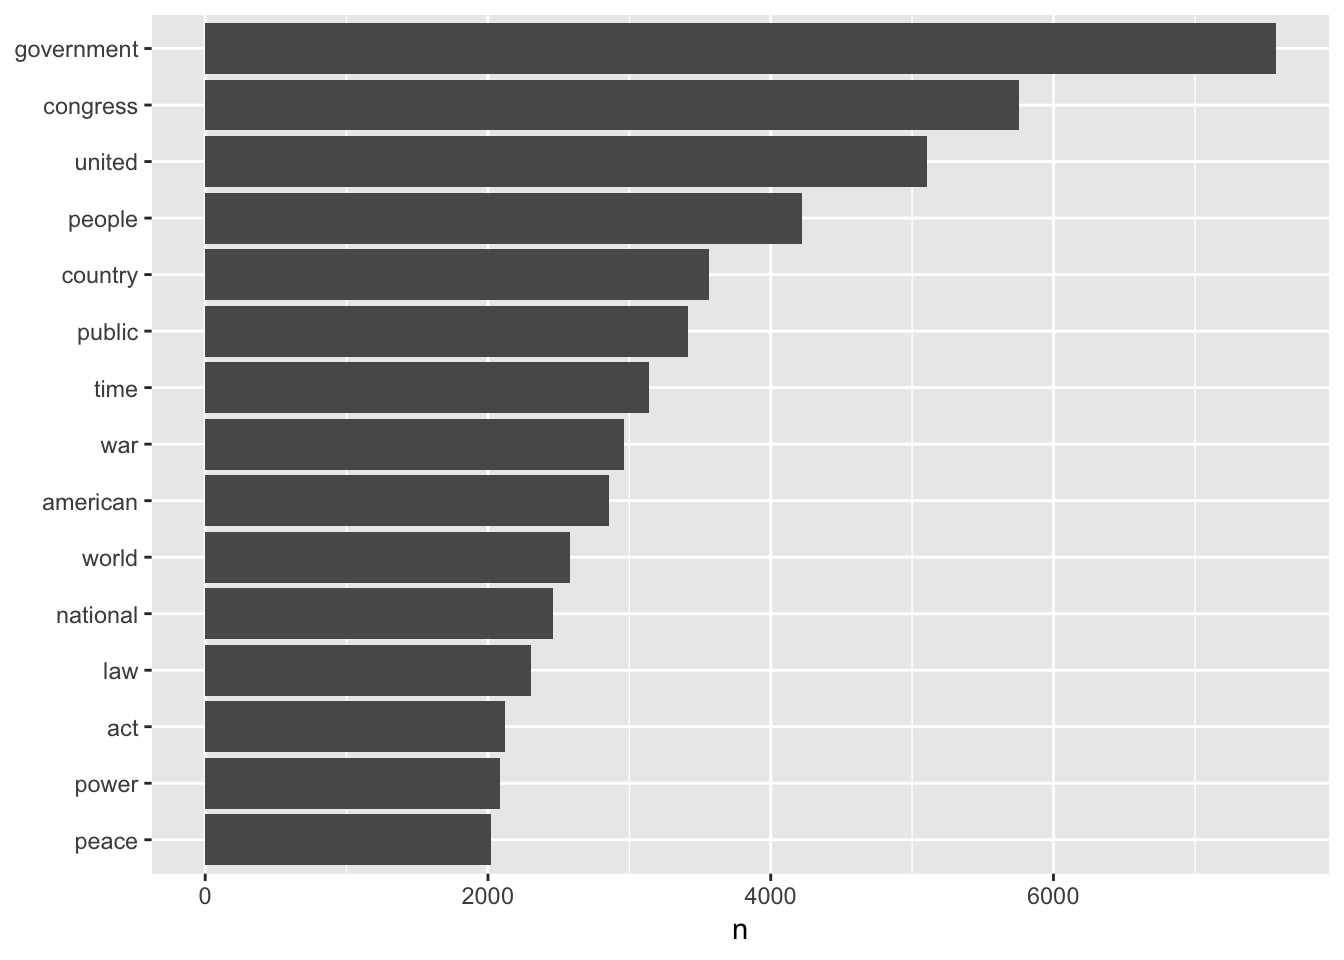
\includegraphics{R-text-analysis_files/figure-latex/unnamed-chunk-14-1.pdf}

What if we're interested in most used words per speech?

\begin{Shaded}
\begin{Highlighting}[]
\CommentTok{# Count words by book}
\NormalTok{doc_words <-}\StringTok{ }\NormalTok{tidy_sotu_words }\OperatorTok
\StringTok{  }\KeywordTok{count}\NormalTok{(doc_id, word, }\DataTypeTok{sort =} \OtherTok{TRUE}\NormalTok{)}

\CommentTok{# Calculate the total number of words by book and save them to a tibble}
\NormalTok{total_words <-}\StringTok{ }\NormalTok{doc_words }\OperatorTok
\StringTok{  }\KeywordTok{group_by}\NormalTok{(doc_id) }\OperatorTok
\StringTok{  }\KeywordTok{summarize}\NormalTok{(}\DataTypeTok{total =} \KeywordTok{sum}\NormalTok{(n))}

\CommentTok{# Join the total column with the rest of the data so we can calculate frequency}
\NormalTok{doc_words <-}\StringTok{ }\KeywordTok{left_join}\NormalTok{(doc_words, total_words)}
\end{Highlighting}
\end{Shaded}

\begin{verbatim}
#> Joining, by = "doc_id"
\end{verbatim}

\begin{Shaded}
\begin{Highlighting}[]
\NormalTok{doc_words }
\end{Highlighting}
\end{Shaded}

Let's graph the top words per book

\begin{Shaded}
\begin{Highlighting}[]
\NormalTok{doc_words }\OperatorTok\StringTok{ }
\StringTok{  }\KeywordTok{filter}\NormalTok{(n }\OperatorTok{>}\StringTok{ }\DecValTok{100}\NormalTok{) }\OperatorTok
\StringTok{  }\KeywordTok{ggplot}\NormalTok{(}\KeywordTok{aes}\NormalTok{(word, n, }\DataTypeTok{fill =}\NormalTok{ doc_id)) }\OperatorTok{+}
\StringTok{  }\KeywordTok{geom_col}\NormalTok{() }\OperatorTok{+}\StringTok{ }
\StringTok{  }\KeywordTok{xlab}\NormalTok{(}\OtherTok{NULL}\NormalTok{) }\OperatorTok{+}
\StringTok{  }\KeywordTok{coord_flip}\NormalTok{()}
\end{Highlighting}
\end{Shaded}

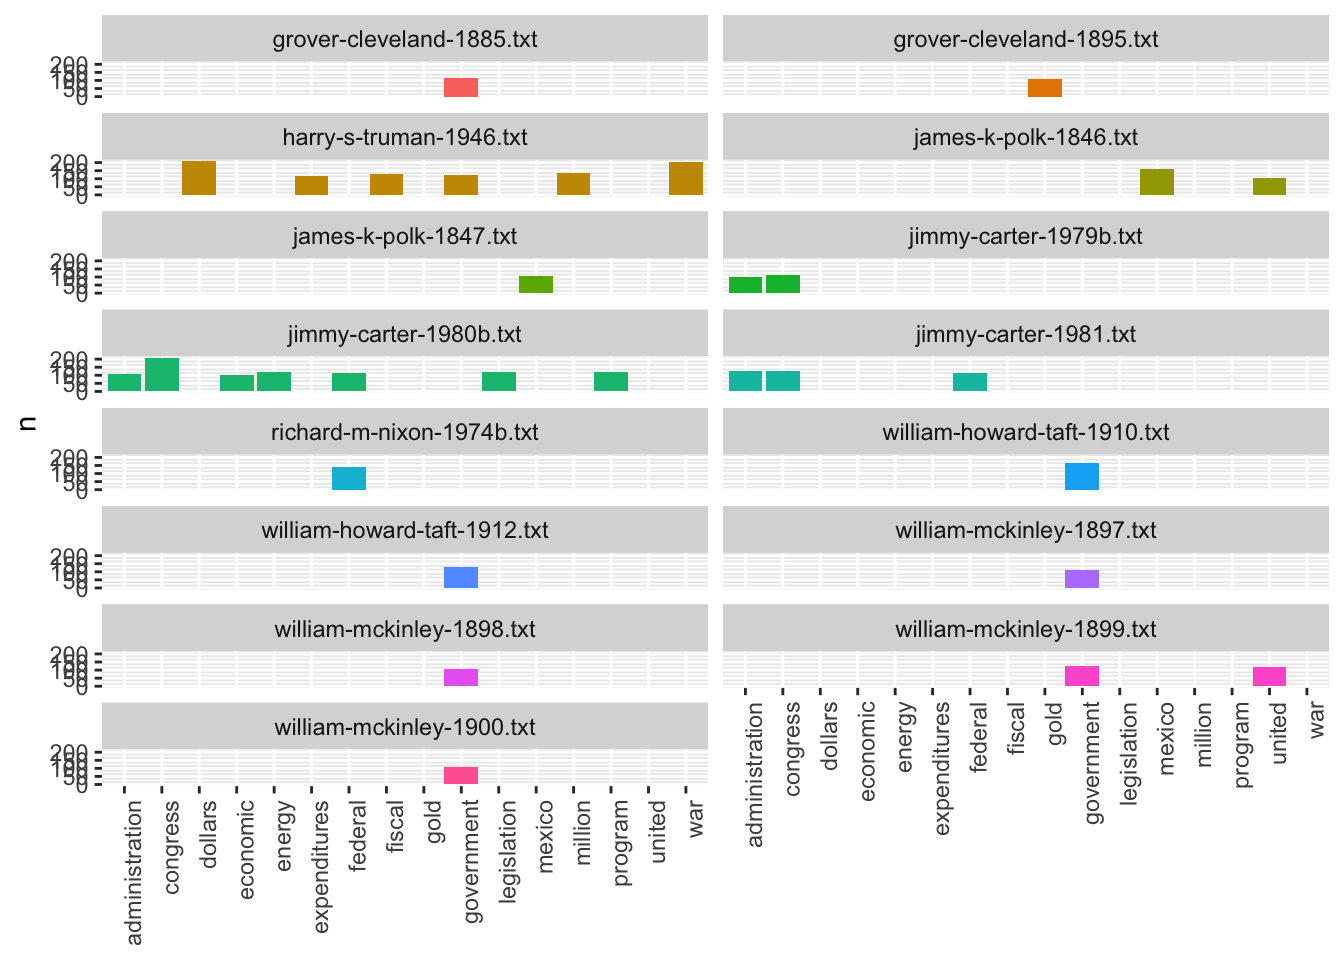
\includegraphics{R-text-analysis_files/figure-latex/unnamed-chunk-16-1.pdf}

That's cool looking, but let's split it into facets so we can see by speech.

\begin{Shaded}
\begin{Highlighting}[]
\NormalTok{doc_words }\OperatorTok\StringTok{ }
\StringTok{  }\KeywordTok{filter}\NormalTok{(n }\OperatorTok{>}\StringTok{ }\DecValTok{100}\NormalTok{) }\OperatorTok
\StringTok{  }\KeywordTok{ggplot}\NormalTok{(}\KeywordTok{aes}\NormalTok{(word, n, }\DataTypeTok{fill =}\NormalTok{ doc_id)) }\OperatorTok{+}
\StringTok{  }\KeywordTok{geom_col}\NormalTok{(}\DataTypeTok{show.legend =} \OtherTok{FALSE}\NormalTok{) }\OperatorTok{+}\StringTok{ }
\StringTok{  }\KeywordTok{xlab}\NormalTok{(}\OtherTok{NULL}\NormalTok{) }\OperatorTok{+}
\StringTok{  }\KeywordTok{facet_wrap}\NormalTok{(}\OperatorTok{~}\NormalTok{doc_id, }\DataTypeTok{ncol =} \DecValTok{2}\NormalTok{) }\OperatorTok{+}\StringTok{ }
\StringTok{  }\KeywordTok{theme}\NormalTok{(}\DataTypeTok{axis.text.x =} \KeywordTok{element_text}\NormalTok{(}\DataTypeTok{angle =} \DecValTok{90}\NormalTok{, }\DataTypeTok{hjust =} \DecValTok{1}\NormalTok{))}
\end{Highlighting}
\end{Shaded}

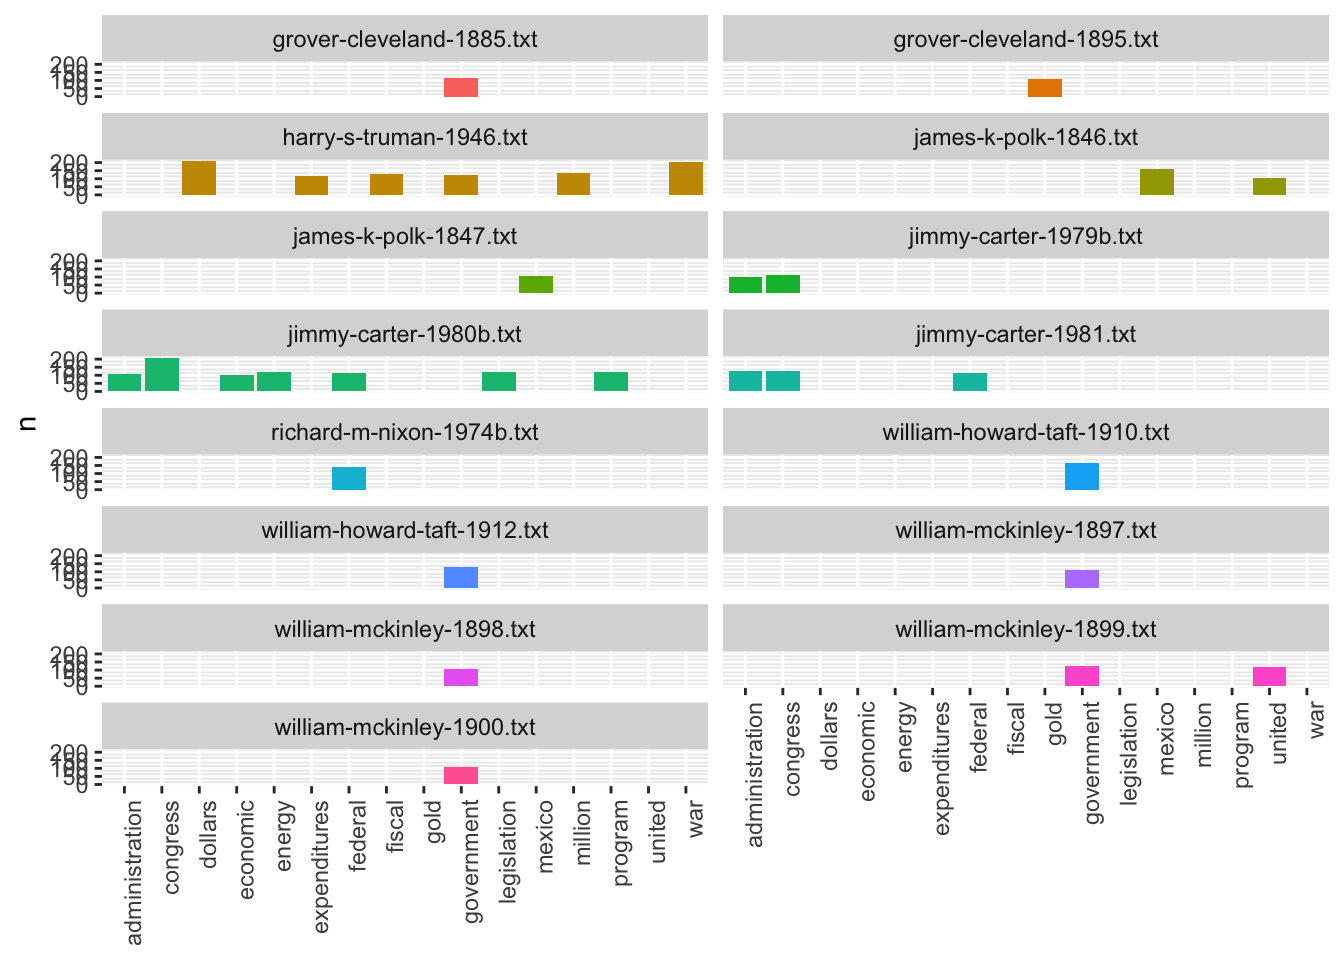
\includegraphics{R-text-analysis_files/figure-latex/unnamed-chunk-17-1.pdf}

We could keep cleaning this figure up by setting some minimum sizing, determining the spacing between y-axis labels better, and so forth, but now we'll accept it as showing some sense of variation across speeches where certain words are used most.

What if we want to check the most highly common words per speech for a single president? We could filter this \texttt{doc\_words} dataset based on the president's name being in the doc\_id, but I think it's easier to filter from the initial tidy data and recount.

\begin{Shaded}
\begin{Highlighting}[]
\NormalTok{tidy_sotu_words }\OperatorTok
\StringTok{  }\KeywordTok{filter}\NormalTok{(president }\OperatorTok{==}\StringTok{ "Barack Obama"}\NormalTok{) }\OperatorTok
\StringTok{  }\KeywordTok{count}\NormalTok{(doc_id, word, }\DataTypeTok{sort =} \OtherTok{TRUE}\NormalTok{) }\OperatorTok
\StringTok{  }\KeywordTok{filter}\NormalTok{(n }\OperatorTok{>}\StringTok{ }\DecValTok{20}\NormalTok{) }\OperatorTok
\StringTok{  }\KeywordTok{ggplot}\NormalTok{(}\KeywordTok{aes}\NormalTok{(word, n, }\DataTypeTok{fill=}\NormalTok{doc_id)) }\OperatorTok{+}
\StringTok{  }\KeywordTok{geom_col}\NormalTok{() }\OperatorTok{+}
\StringTok{  }\KeywordTok{facet_wrap}\NormalTok{(}\OperatorTok{~}\NormalTok{doc_id, }\DataTypeTok{ncol =} \DecValTok{2}\NormalTok{) }\OperatorTok{+}\StringTok{ }
\StringTok{  }\KeywordTok{theme}\NormalTok{(}\DataTypeTok{axis.text.x =} \KeywordTok{element_text}\NormalTok{(}\DataTypeTok{angle =} \DecValTok{90}\NormalTok{, }\DataTypeTok{hjust =} \DecValTok{1}\NormalTok{))}
\end{Highlighting}
\end{Shaded}

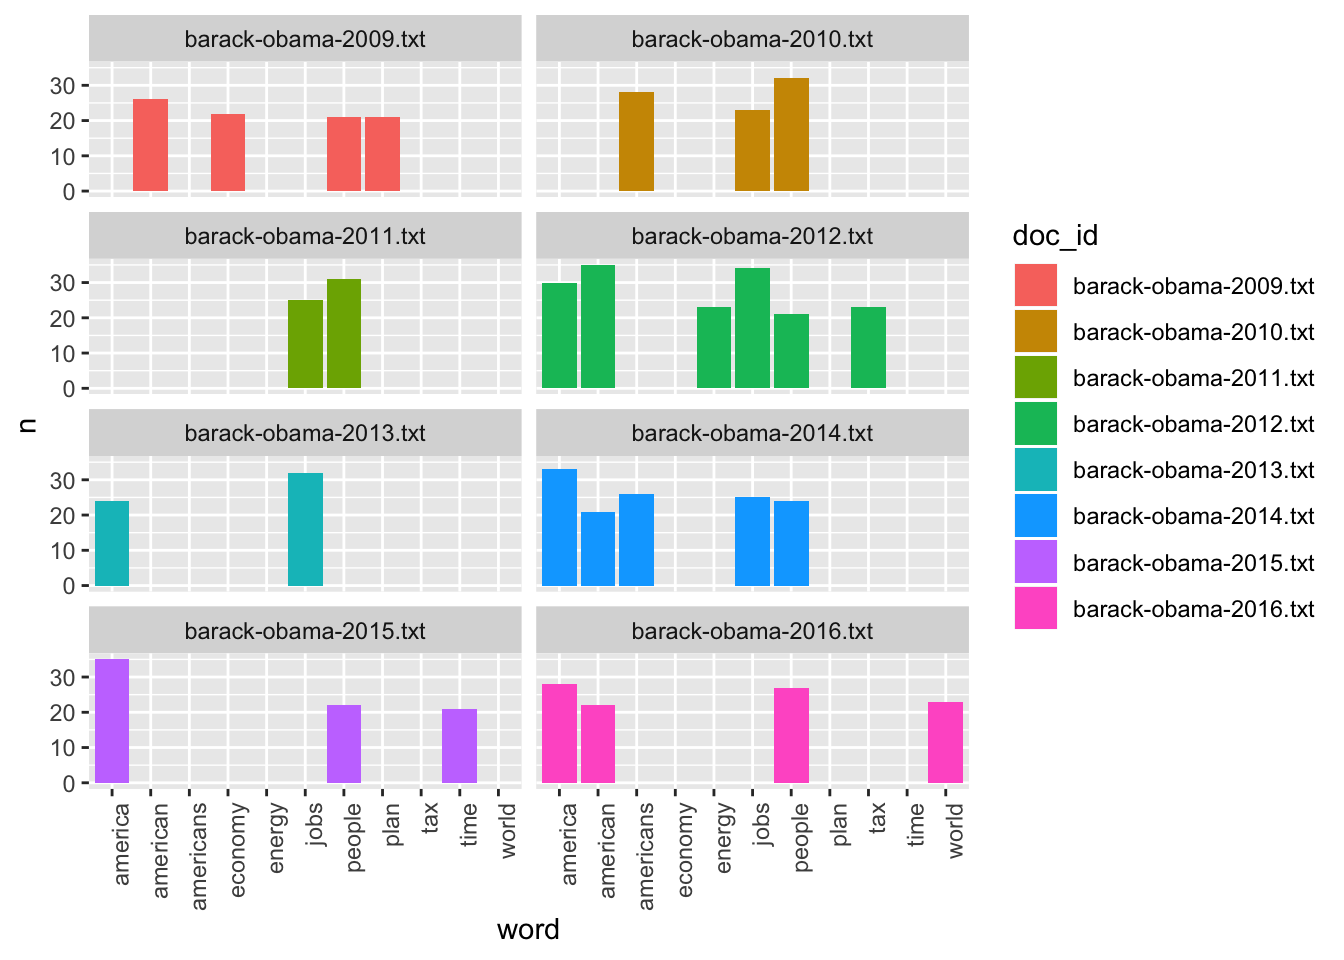
\includegraphics{R-text-analysis_files/figure-latex/unnamed-chunk-18-1.pdf}

\hypertarget{term-frequency}{%
\section{Term frequency}\label{term-frequency}}

Sometimes, a raw count of a word is less important than understanding how often that word appears in respect to the total number of words in a text. This ratio would be the \textbf{term frequency}.

\begin{Shaded}
\begin{Highlighting}[]
\NormalTok{doc_words <-}\StringTok{ }\NormalTok{doc_words }\OperatorTok
\StringTok{  }\KeywordTok{mutate}\NormalTok{(}\DataTypeTok{term_freq =}\NormalTok{ n }\OperatorTok{/}\StringTok{ }\NormalTok{total)}

\NormalTok{doc_words }
\end{Highlighting}
\end{Shaded}

Let's graph the term frequency for one of these speeches so we can understand the frequency distribution of words over a text.

\begin{Shaded}
\begin{Highlighting}[]
\NormalTok{doc_words }\OperatorTok
\StringTok{  }\KeywordTok{filter}\NormalTok{(doc_id }\OperatorTok{==}\StringTok{ "harry-s-truman-1946.txt"}\NormalTok{) }\OperatorTok
\StringTok{  }\KeywordTok{ggplot}\NormalTok{(}\KeywordTok{aes}\NormalTok{(term_freq)) }\OperatorTok{+}
\StringTok{  }\KeywordTok{geom_histogram}\NormalTok{(}\DataTypeTok{show.legend =} \OtherTok{FALSE}\NormalTok{) }\OperatorTok{+}
\StringTok{  }\KeywordTok{xlim}\NormalTok{(}\OtherTok{NA}\NormalTok{, }\FloatTok{.012}\NormalTok{)}
\end{Highlighting}
\end{Shaded}

\begin{verbatim}
#> `stat_bin()` using `bins = 30`. Pick better value with `binwidth`.
\end{verbatim}

\begin{verbatim}
#> Warning: Removed 2 rows containing non-finite values (stat_bin).
\end{verbatim}

\begin{verbatim}
#> Warning: Removed 1 rows containing missing values (geom_bar).
\end{verbatim}

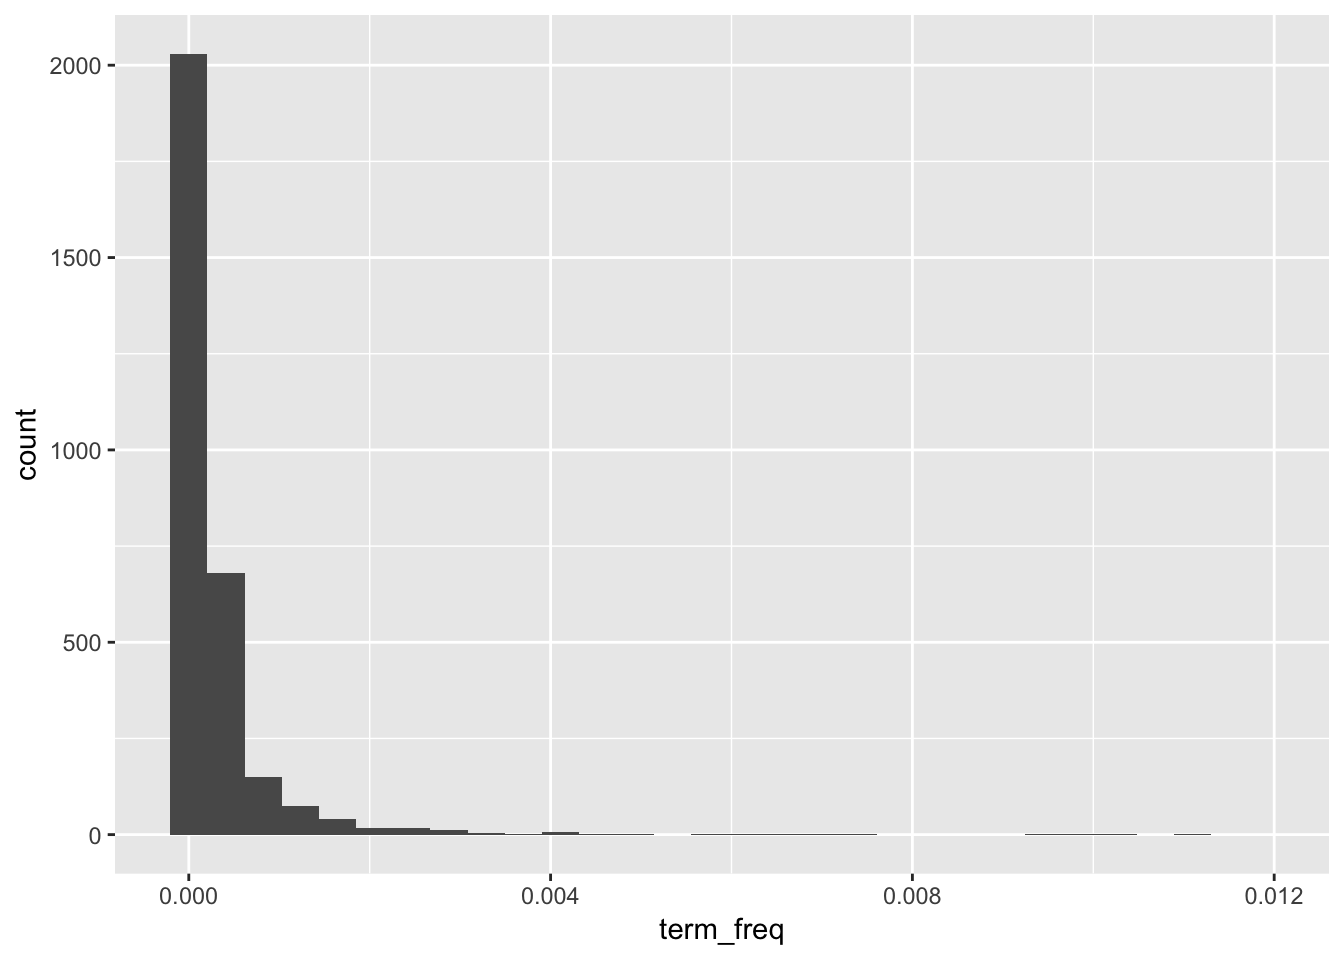
\includegraphics{R-text-analysis_files/figure-latex/unnamed-chunk-20-1.pdf}

This should make sense. Most words are used relatively rarely in a text. Only a few have a high term frequency.

We could keep filtering this data to see which terms have the high frequency, thus maybe increased significance, for different presidents and different particular speeches. We could also subset based on decade, and get a sense of what was important in each decade. We're going to take a slightly different approach though. We've been looking at term frequency per document. What if we want to know about words that seem more important based on the contents of the entire corpus?

\hypertarget{tf-idf}{%
\section{Tf-idf}\label{tf-idf}}

For this, we can use term-frequency according to inverse document frequency (tf-idf). Tf-idf meansures how important a word is within a corpus by scaling term frequency per document according to the inverse of the term's document frequency (how many documents within the corpus in which the term appears divided by the number of documents).

We could write our own function for tf-idf, but in this case we'll take advantage of tidytext's implementation.

\begin{Shaded}
\begin{Highlighting}[]
\NormalTok{doc_words <-}\StringTok{ }\NormalTok{doc_words }\OperatorTok
\StringTok{  }\KeywordTok{bind_tf_idf}\NormalTok{(word, doc_id, n)}

\NormalTok{doc_words}
\end{Highlighting}
\end{Shaded}

The tf-idf value will be:

\begin{itemize}
\tightlist
\item
  lower for words that appear in many documents in the corpus, and lowest when the word occurs in virtually all documents.
\item
  high for words that appear many times in few documents in the corpus, this lending high discrimiatory power to those doucments.
\end{itemize}

Let's look at some of the words in the corpus that have the highest tf-idf scores, which means words that are particularly distinctive for their documents.

\begin{Shaded}
\begin{Highlighting}[]
\NormalTok{doc_words }\OperatorTok
\StringTok{  }\KeywordTok{select}\NormalTok{(}\OperatorTok{-}\NormalTok{total) }\OperatorTok
\StringTok{  }\KeywordTok{arrange}\NormalTok{(}\KeywordTok{desc}\NormalTok{(tf_idf))}
\end{Highlighting}
\end{Shaded}

These results seem appropriate given our history. To understand the occurence of the years we might need to look more closely at the speeches themselves, and determine whether the years are significant or whether they need to be removed from the text. It might be that even if they don't need to be removed from the text overall, they still need to be filtered out within the context of this analysis.

In the same way that we narrowed our analysis to Obama speeches earlier, we could subset the corpus before we calculate the tf-idf score to understand which words are most important for a single president within their sotu speeches. Let's do that for Obama.

\begin{Shaded}
\begin{Highlighting}[]
\NormalTok{obama_tf_idf <-}\StringTok{ }\NormalTok{tidy_sotu_words }\OperatorTok
\StringTok{  }\KeywordTok{filter}\NormalTok{(president }\OperatorTok{==}\StringTok{ "Barack Obama"}\NormalTok{) }\OperatorTok
\StringTok{  }\KeywordTok{count}\NormalTok{(doc_id, word, }\DataTypeTok{sort =} \OtherTok{TRUE}\NormalTok{) }\OperatorTok
\StringTok{  }\KeywordTok{bind_tf_idf}\NormalTok{(word, doc_id, n) }\OperatorTok
\StringTok{  }\KeywordTok{arrange}\NormalTok{(}\KeywordTok{desc}\NormalTok{(tf_idf))}

\NormalTok{obama_tf_idf}
\end{Highlighting}
\end{Shaded}

Based on what you know of the Obama years and sotu speeches generally, how would you interpret these results?

Let's try graphing these results, showing the top tf-idf terms per speech for Obama's speeches.

\begin{Shaded}
\begin{Highlighting}[]
\NormalTok{obama_tf_idf }\OperatorTok
\StringTok{  }\KeywordTok{group_by}\NormalTok{(doc_id) }\OperatorTok
\StringTok{  }\KeywordTok{mutate}\NormalTok{(}\DataTypeTok{word =} \KeywordTok{factor}\NormalTok{(word, }\DataTypeTok{levels =} \KeywordTok{rev}\NormalTok{(}\KeywordTok{unique}\NormalTok{(word)))) }\OperatorTok\StringTok{ }
\StringTok{  }\KeywordTok{group_by}\NormalTok{(doc_id) }\OperatorTok\StringTok{ }
\StringTok{  }\KeywordTok{top_n}\NormalTok{(}\DecValTok{5}\NormalTok{) }\OperatorTok\StringTok{ }
\StringTok{  }\KeywordTok{ungroup}\NormalTok{() }\OperatorTok
\StringTok{  }\KeywordTok{ggplot}\NormalTok{(}\KeywordTok{aes}\NormalTok{(word, tf_idf, }\DataTypeTok{fill =}\NormalTok{ doc_id)) }\OperatorTok{+}
\StringTok{  }\KeywordTok{geom_col}\NormalTok{(}\DataTypeTok{show.legend =} \OtherTok{FALSE}\NormalTok{) }\OperatorTok{+}
\StringTok{  }\KeywordTok{labs}\NormalTok{(}\DataTypeTok{x =} \OtherTok{NULL}\NormalTok{, }\DataTypeTok{y =} \StringTok{"tf-idf"}\NormalTok{) }\OperatorTok{+}
\StringTok{  }\KeywordTok{facet_wrap}\NormalTok{(}\OperatorTok{~}\NormalTok{doc_id, }\DataTypeTok{ncol =} \DecValTok{2}\NormalTok{, }\DataTypeTok{scales =} \StringTok{"free"}\NormalTok{) }\OperatorTok{+}
\StringTok{  }\KeywordTok{coord_flip}\NormalTok{() }\OperatorTok{+}\StringTok{ }
\StringTok{  }\KeywordTok{theme}\NormalTok{(}\DataTypeTok{axis.text.y =} \KeywordTok{element_text}\NormalTok{(}\DataTypeTok{angle =} \DecValTok{45}\NormalTok{)) }
\end{Highlighting}
\end{Shaded}

\begin{verbatim}
#> Warning in mutate_impl(.data, dots): Unequal factor levels: coercing to
#> character
\end{verbatim}

\begin{verbatim}
#> Warning in mutate_impl(.data, dots): binding character and factor vector,
#> coercing into character vector

#> Warning in mutate_impl(.data, dots): binding character and factor vector,
#> coercing into character vector

#> Warning in mutate_impl(.data, dots): binding character and factor vector,
#> coercing into character vector

#> Warning in mutate_impl(.data, dots): binding character and factor vector,
#> coercing into character vector

#> Warning in mutate_impl(.data, dots): binding character and factor vector,
#> coercing into character vector

#> Warning in mutate_impl(.data, dots): binding character and factor vector,
#> coercing into character vector

#> Warning in mutate_impl(.data, dots): binding character and factor vector,
#> coercing into character vector

#> Warning in mutate_impl(.data, dots): binding character and factor vector,
#> coercing into character vector
\end{verbatim}

\begin{verbatim}
#> Selecting by tf_idf
\end{verbatim}

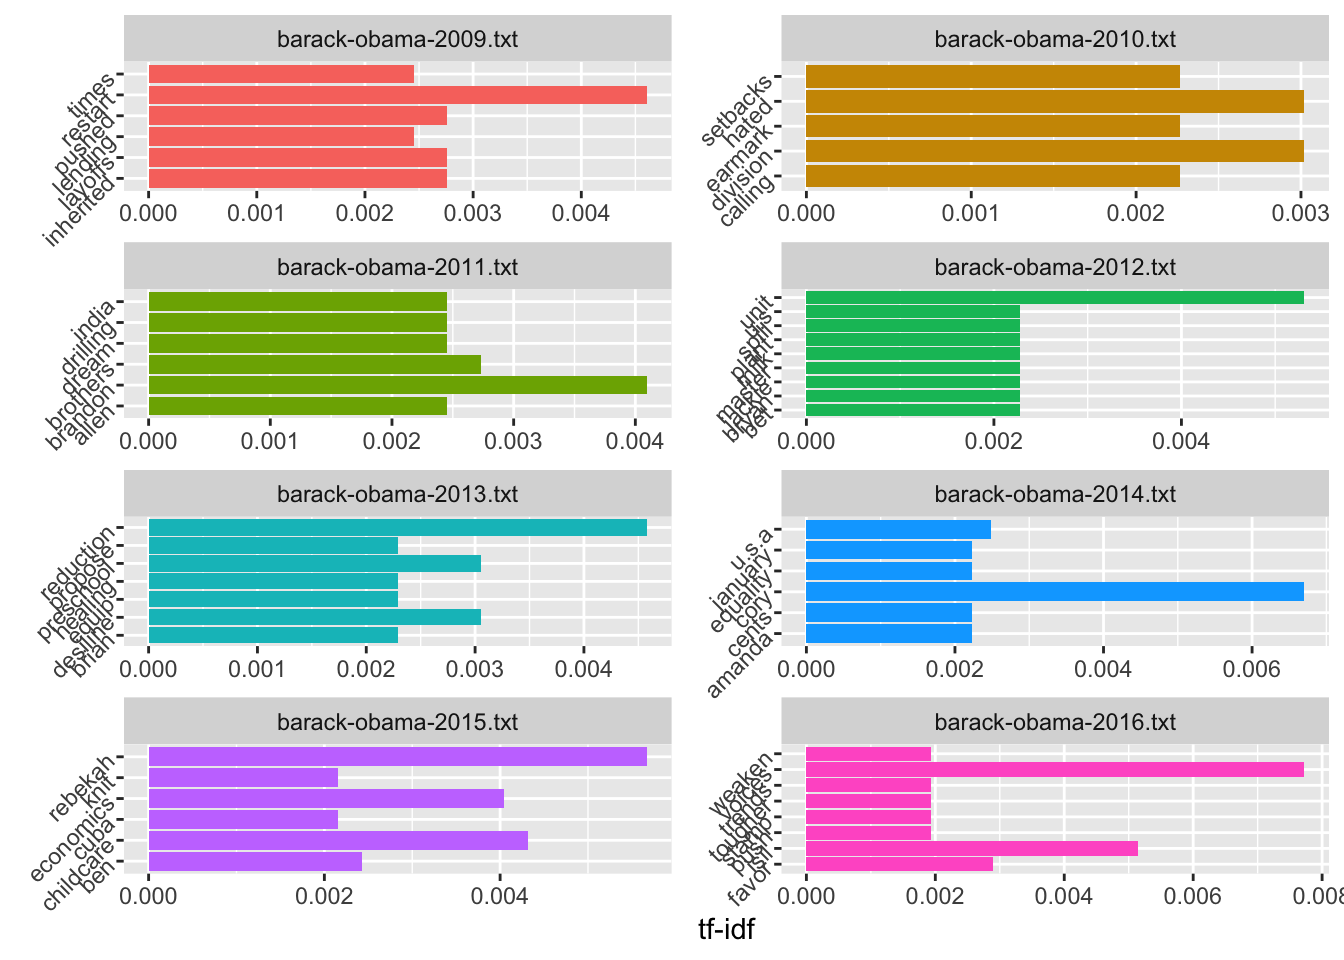
\includegraphics{R-text-analysis_files/figure-latex/unnamed-chunk-24-1.pdf}

\hypertarget{n-grams}{%
\section{N-Grams}\label{n-grams}}

\url{https://www.tidytextmining.com/ngrams.html\#counting-and-correlating-pairs-of-words-with-the-widyr-package}
We have mentioned n-grams in the intro, let's revisit this here and take a look at the most common bigrams in the speeches. Remember this is what we get back:

\begin{Shaded}
\begin{Highlighting}[]
\NormalTok{sotu_whole }\OperatorTok
\StringTok{  }\KeywordTok{unnest_tokens}\NormalTok{(bigram, text, }\DataTypeTok{token =} \StringTok{"ngrams"}\NormalTok{, }\DataTypeTok{n =} \DecValTok{2}\NormalTok{) }\CommentTok{# create bigram}
\end{Highlighting}
\end{Shaded}

Let's see the most common bigrams:

\begin{Shaded}
\begin{Highlighting}[]
\NormalTok{sotu_whole }\OperatorTok
\StringTok{  }\KeywordTok{unnest_tokens}\NormalTok{(bigram, text, }\DataTypeTok{token =} \StringTok{"ngrams"}\NormalTok{, }\DataTypeTok{n =} \DecValTok{2}\NormalTok{) }\OperatorTok\StringTok{ }
\StringTok{  }\KeywordTok{count}\NormalTok{(bigram, }\DataTypeTok{sort =} \OtherTok{TRUE}\NormalTok{) }\CommentTok{# count ocurrences and sord descending}
\end{Highlighting}
\end{Shaded}

Ok, so we again need to remove the stopwords. This time let's use dplyr's \texttt{filter} function for this. And before that we will \texttt{separate} the two words into two columns.

\begin{Shaded}
\begin{Highlighting}[]
\NormalTok{sotu_bigrams <-}\StringTok{ }\NormalTok{sotu_whole }\OperatorTok
\StringTok{  }\KeywordTok{unnest_tokens}\NormalTok{(bigram, text, }\DataTypeTok{token =} \StringTok{"ngrams"}\NormalTok{, }\DataTypeTok{n =} \DecValTok{2}\NormalTok{) }\OperatorTok\StringTok{ }
\StringTok{  }\KeywordTok{separate}\NormalTok{(bigram, }\KeywordTok{c}\NormalTok{(}\StringTok{"word1"}\NormalTok{, }\StringTok{"word2"}\NormalTok{), }\DataTypeTok{sep =} \StringTok{" "}\NormalTok{) }\OperatorTok\StringTok{ }\CommentTok{# separate into cols}
\StringTok{  }\KeywordTok{filter}\NormalTok{(}\OperatorTok{!}\NormalTok{word1 }\OperatorTok\StringTok{ }\NormalTok{stop_words}\OperatorTok{$}\NormalTok{word) }\OperatorTok\StringTok{ }\CommentTok{# remove stopwords}
\StringTok{  }\KeywordTok{filter}\NormalTok{(}\OperatorTok{!}\NormalTok{word2 }\OperatorTok\StringTok{ }\NormalTok{stop_words}\OperatorTok{$}\NormalTok{word)}

\NormalTok{sotu_bigrams }\OperatorTok\StringTok{ }
\StringTok{  }\KeywordTok{count}\NormalTok{(word1, word2, }\DataTypeTok{sort =} \OtherTok{TRUE}\NormalTok{)}
\end{Highlighting}
\end{Shaded}

(Bonus question: What happened on that June 30th?)

A bigram can also be treated as a term in a document in the same way that we treated individual words. That means we can look at tf-idf values in the same way.

First we will re-unite the two word columns again, and then generate the tf-idf count as above.

\begin{Shaded}
\begin{Highlighting}[]
\NormalTok{bigram_tf_idf <-}\StringTok{ }\NormalTok{sotu_bigrams }\OperatorTok
\StringTok{  }\KeywordTok{unite}\NormalTok{(bigram, word1, word2, }\DataTypeTok{sep =} \StringTok{" "}\NormalTok{) }\OperatorTok\StringTok{ }\CommentTok{# combine columns}
\StringTok{  }\KeywordTok{count}\NormalTok{(president, bigram) }\OperatorTok
\StringTok{  }\KeywordTok{bind_tf_idf}\NormalTok{(bigram, president, n) }\OperatorTok
\StringTok{  }\KeywordTok{arrange}\NormalTok{(}\KeywordTok{desc}\NormalTok{(tf_idf))}
\end{Highlighting}
\end{Shaded}

What makes the speeches of different presidents unique?

Let's pick a few presidents and plot their highest scoreing tf-idf values here.

\begin{Shaded}
\begin{Highlighting}[]
\NormalTok{potus <-}\StringTok{ }\KeywordTok{c}\NormalTok{(}\StringTok{"John F. Kennedy"}\NormalTok{, }\StringTok{"Richard M. Nixon"}\NormalTok{, }\StringTok{"William J. Clinton"}\NormalTok{, }\StringTok{"George Bush"}\NormalTok{, }\StringTok{"George W. Bush"}\NormalTok{, }\StringTok{"Jimmy Carter"}\NormalTok{)}

\NormalTok{bigram_tf_idf }\OperatorTok
\StringTok{  }\KeywordTok{filter}\NormalTok{(president }\OperatorTok\StringTok{ }\NormalTok{potus) }\OperatorTok\StringTok{ }
\StringTok{  }\KeywordTok{group_by}\NormalTok{(president) }\OperatorTok\StringTok{ }
\StringTok{  }\KeywordTok{top_n}\NormalTok{(}\DecValTok{20}\NormalTok{) }\OperatorTok\StringTok{ }
\StringTok{  }\KeywordTok{ggplot}\NormalTok{(}\KeywordTok{aes}\NormalTok{(}\KeywordTok{reorder}\NormalTok{(bigram, tf_idf), tf_idf, }\DataTypeTok{fill =}\NormalTok{ president)) }\OperatorTok{+}
\StringTok{  }\KeywordTok{geom_col}\NormalTok{(}\DataTypeTok{show.legend =} \OtherTok{FALSE}\NormalTok{) }\OperatorTok{+}
\StringTok{  }\KeywordTok{labs}\NormalTok{(}\DataTypeTok{x =} \OtherTok{NULL}\NormalTok{, }\DataTypeTok{y =} \StringTok{"tf-idf"}\NormalTok{) }\OperatorTok{+}
\StringTok{  }\KeywordTok{facet_wrap}\NormalTok{(}\OperatorTok{~}\NormalTok{president, }\DataTypeTok{scales =} \StringTok{"free"}\NormalTok{, }\DataTypeTok{nrow =} \DecValTok{2}\NormalTok{) }\OperatorTok{+}
\StringTok{  }\KeywordTok{coord_flip}\NormalTok{()}
\end{Highlighting}
\end{Shaded}

\begin{verbatim}
#> Selecting by tf_idf
\end{verbatim}

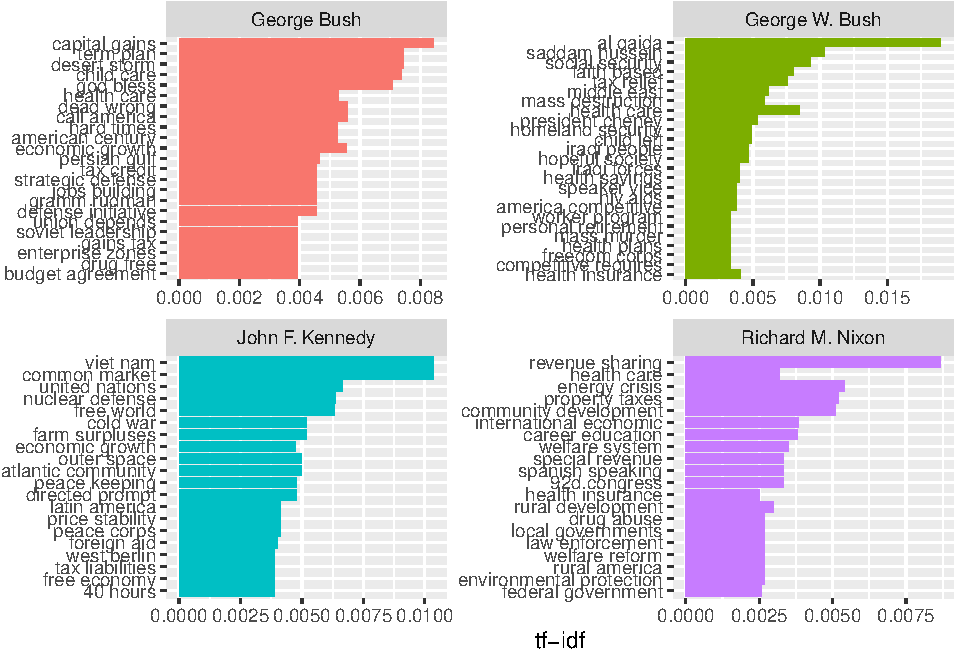
\includegraphics{R-text-analysis_files/figure-latex/bigram-tf-idf-plot-1.pdf}

\hypertarget{co-ocurrcence}{%
\section{Co-ocurrcence}\label{co-ocurrcence}}

Co-occurances give us a sense of words that appear in the same text, but not necessarily next to each other.

For this section we will make use of the \texttt{widyr} package. It allows us to turn our table into a wide matrix. In our case that matrix will be made up of the individual words and the cell values will be the counts of how many times they co-occur. Then we will turn the matrix back into a tidy form, where each row contains the word pairs and the count of their co-occurrence. This lets us count common pairs of words co-appearing within the same speech.

The function which helps us do this is the \texttt{pairwise\_count()} function.

Since processing the entire corpus would take too long here, we will only look at the last 20 words of each speech.

\begin{Shaded}
\begin{Highlighting}[]
\KeywordTok{library}\NormalTok{(widyr)}

\CommentTok{# extract last 100 words from text}
\NormalTok{sotu_whole}\OperatorTok{$}\NormalTok{speech_end <-}\StringTok{ }\KeywordTok{word}\NormalTok{(sotu_whole}\OperatorTok{$}\NormalTok{text, }\DecValTok{-100}\NormalTok{, }\DataTypeTok{end =} \DecValTok{-1}\NormalTok{)}

\NormalTok{sotu_word_pairs <-}\StringTok{ }\NormalTok{sotu_whole }\OperatorTok\StringTok{ }
\StringTok{  }\KeywordTok{unnest_tokens}\NormalTok{(word, speech_end) }\OperatorTok\StringTok{ }
\StringTok{  }\KeywordTok{filter}\NormalTok{(}\OperatorTok{!}\NormalTok{word }\OperatorTok\StringTok{ }\NormalTok{stop_words}\OperatorTok{$}\NormalTok{word) }\OperatorTok\StringTok{ }\CommentTok{# remove stopwords}
\StringTok{  }\KeywordTok{pairwise_count}\NormalTok{(word, doc_id, }\DataTypeTok{sort =} \OtherTok{TRUE}\NormalTok{, }\DataTypeTok{upper =} \OtherTok{FALSE}\NormalTok{) }\CommentTok{# don't include upper triangle of matrix}
\end{Highlighting}
\end{Shaded}

To plot the co-ocurrcance network, we use the \texttt{igraph} library to convert our table into a network graph and \texttt{ggraph} which adds functionality to ggplot and makes it easier create a network plot.

\begin{Shaded}
\begin{Highlighting}[]
\KeywordTok{library}\NormalTok{(igraph)}
\KeywordTok{library}\NormalTok{(ggraph)}

\NormalTok{sotu_word_pairs }\OperatorTok\StringTok{ }
\StringTok{  }\KeywordTok{filter}\NormalTok{(n }\OperatorTok{>=}\StringTok{ }\DecValTok{10}\NormalTok{) }\OperatorTok\StringTok{  }\CommentTok{# only word pairs that occur 10 or more times}
\StringTok{  }\KeywordTok{graph_from_data_frame}\NormalTok{() }\OperatorTok\StringTok{ }\CommentTok{#convert to graph}
\StringTok{  }\KeywordTok{ggraph}\NormalTok{(}\DataTypeTok{layout =} \StringTok{"fr"}\NormalTok{) }\OperatorTok{+}\StringTok{ }\CommentTok{# place nodes according to the force-directed algorithm of Fruchterman and Reingold}
\StringTok{  }\KeywordTok{geom_edge_link}\NormalTok{(}\KeywordTok{aes}\NormalTok{(}\DataTypeTok{edge_alpha =}\NormalTok{ n, }\DataTypeTok{edge_width =}\NormalTok{ n), }\DataTypeTok{edge_colour =} \StringTok{"tomato"}\NormalTok{) }\OperatorTok{+}
\StringTok{  }\KeywordTok{geom_node_point}\NormalTok{(}\DataTypeTok{size =} \DecValTok{5}\NormalTok{) }\OperatorTok{+}
\StringTok{  }\KeywordTok{geom_node_text}\NormalTok{(}\KeywordTok{aes}\NormalTok{(}\DataTypeTok{label =}\NormalTok{ name), }\DataTypeTok{repel =} \OtherTok{TRUE}\NormalTok{, }
                 \DataTypeTok{point.padding =} \KeywordTok{unit}\NormalTok{(}\FloatTok{0.2}\NormalTok{, }\StringTok{"lines"}\NormalTok{)) }\OperatorTok{+}
\StringTok{  }\KeywordTok{theme_void}\NormalTok{()}
\end{Highlighting}
\end{Shaded}

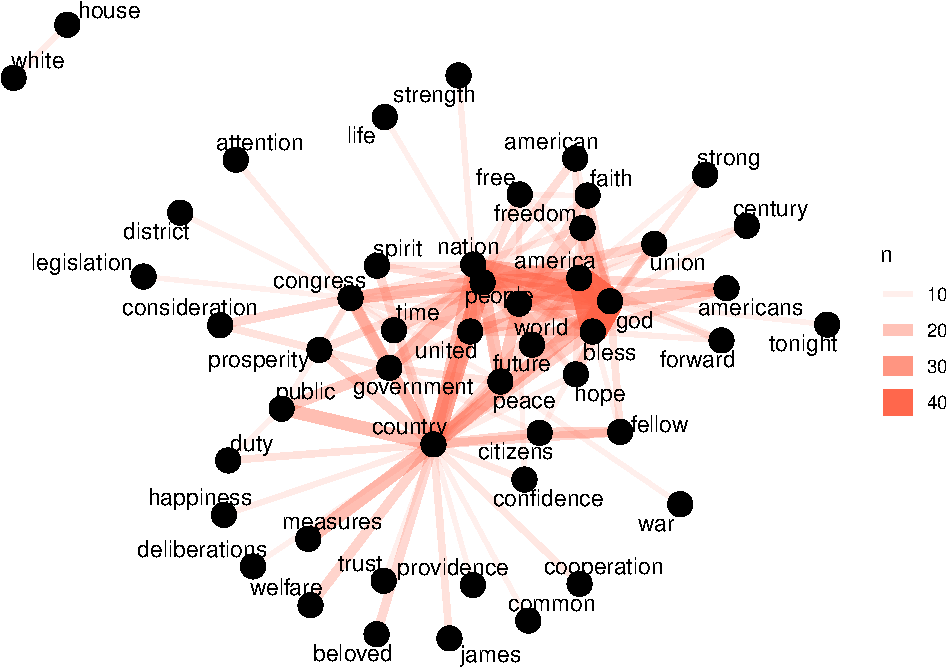
\includegraphics{R-text-analysis_files/figure-latex/plot-network-1.pdf}

There are alternative approaches for this as well. See for example the \texttt{findAssocs} function in the \texttt{tm} package.

\hypertarget{document-term-matrix}{%
\section{Document-Term Matrix}\label{document-term-matrix}}

A \href{https://en.wikipedia.org/wiki/Document-term_matrix}{document-term matrix (DTM)} is a format which is frequently used in textanalysis. It is a matrix where we can see the counts of each term per document. In a DTM each row represents a document, each column represents a term, and the cell values are the counts of the ocurrences of the term for the particular document.

\texttt{tidytext} provides functionality to convert to and from DTMs, if for example, your analyis requires specific functions that require you to use a different R package which only works with DTM objects.

The \texttt{cast\_dtm} function can be used to create a DTM object from a tidy table.

Let's assume that for some reason we want to use the \texttt{findAssoc} function from the \texttt{tm} package.

First we use dplyr to create a table with the document name, the term, and the count.

\begin{Shaded}
\begin{Highlighting}[]
\CommentTok{# make a table with document, term, count}
\NormalTok{tidy_sotu_words }\OperatorTok\StringTok{ }
\StringTok{  }\KeywordTok{count}\NormalTok{(doc_id, word) }
\end{Highlighting}
\end{Shaded}

Now we cast it as a DTM.

\begin{Shaded}
\begin{Highlighting}[]
\NormalTok{sotu_dtm <-}\StringTok{ }\NormalTok{tidy_sotu_words }\OperatorTok\StringTok{ }
\StringTok{  }\KeywordTok{count}\NormalTok{(doc_id, word) }\OperatorTok\StringTok{ }
\StringTok{  }\KeywordTok{cast_dtm}\NormalTok{(doc_id, word, n) }

\KeywordTok{class}\NormalTok{(sotu_dtm)}
\end{Highlighting}
\end{Shaded}

Finally, let's use it in the \texttt{tm} package.

\begin{Shaded}
\begin{Highlighting}[]
\KeywordTok{library}\NormalTok{(tm)}

\CommentTok{# look at the terms with tm function}
\KeywordTok{Terms}\NormalTok{(sotu_dtm) }\OperatorTok\StringTok{ }\KeywordTok{tail}\NormalTok{()}

\CommentTok{# most frequent terms}
\KeywordTok{findFreqTerms}\NormalTok{(sotu_dtm, }\DataTypeTok{lowfreq =} \DecValTok{5000}\NormalTok{)}
              
\CommentTok{# find terms associated with ...}
\KeywordTok{findAssocs}\NormalTok{(sotu_dtm, }\StringTok{"citizen"}\NormalTok{, }\DataTypeTok{corlimit =} \FloatTok{0.5}\NormalTok{)}
\end{Highlighting}
\end{Shaded}

Conversely, \texttt{tidytext} implements the \texttt{tidy} function (originally from the \texttt{broom} package) to import DocumentTermMatrix objects. Note that it only takes the cells from the DTM that are not 0, so there will be no rows with 0 counts.

\hypertarget{sentiment-analysis}{%
\section{Sentiment analysis}\label{sentiment-analysis}}

\texttt{tidytext} comes with a dataset \texttt{sentiments} which contains several sentiment lexicons, where each word is attributed a certain sentiment, like this:

\begin{Shaded}
\begin{Highlighting}[]
\NormalTok{sentiments}
\end{Highlighting}
\end{Shaded}

Here we will take a look at how the sentiment of the speeches change over time. We will use the lexicon from \href{https://www.cs.uic.edu/~liub/FBS/sentiment-analysis.html}{Bing Liu and collaborators}, which assigns positive/negative labels for each word:

\begin{Shaded}
\begin{Highlighting}[]
\NormalTok{bing_lex <-}\StringTok{ }\KeywordTok{get_sentiments}\NormalTok{(}\StringTok{"bing"}\NormalTok{)}
\NormalTok{bing_lex}
\end{Highlighting}
\end{Shaded}

Since this is a regular tibble, we can use these sentiments and join them to the words of our speeches. We will use \texttt{inner\_join} from \texttt{dplyr}. Since our columns to join on have the same name (\texttt{word}) we don't need to explicitly name it.

\begin{Shaded}
\begin{Highlighting}[]
\NormalTok{tidy_sotu_words }\OperatorTok\StringTok{ }
\StringTok{  }\KeywordTok{inner_join}\NormalTok{(bing_lex) }\OperatorTok\StringTok{ }\CommentTok{# join}
\StringTok{  }\KeywordTok{count}\NormalTok{(year, sentiment) }\CommentTok{# group by year and sentiment}
\end{Highlighting}
\end{Shaded}

\begin{verbatim}
#> Joining, by = "word"
\end{verbatim}

Finally we can visualize it like this:

\begin{Shaded}
\begin{Highlighting}[]
\NormalTok{tidy_sotu_words }\OperatorTok\StringTok{ }
\StringTok{  }\KeywordTok{inner_join}\NormalTok{(bing_lex) }\OperatorTok\StringTok{ }\CommentTok{# join}
\StringTok{  }\KeywordTok{count}\NormalTok{(year, sentiment) }\OperatorTok\StringTok{ }\CommentTok{# group by year and sentiment}
\StringTok{  }\KeywordTok{ggplot}\NormalTok{(}\KeywordTok{aes}\NormalTok{(year, n, }\DataTypeTok{color =}\NormalTok{ sentiment)) }\OperatorTok{+}
\StringTok{    }\KeywordTok{geom_line}\NormalTok{() }\OperatorTok{+}
\StringTok{    }\KeywordTok{scale_x_continuous}\NormalTok{(}\DataTypeTok{breaks =} \KeywordTok{seq}\NormalTok{(}\DecValTok{1790}\NormalTok{, }\DecValTok{2016}\NormalTok{, }\DataTypeTok{by =} \DecValTok{10}\NormalTok{)) }\OperatorTok{+}
\StringTok{    }\KeywordTok{theme}\NormalTok{(}\DataTypeTok{axis.text.x =} \KeywordTok{element_text}\NormalTok{(}\DataTypeTok{angle =} \DecValTok{45}\NormalTok{, }\DataTypeTok{hjust =} \DecValTok{1}\NormalTok{))}
\end{Highlighting}
\end{Shaded}

\begin{verbatim}
#> Joining, by = "word"
\end{verbatim}

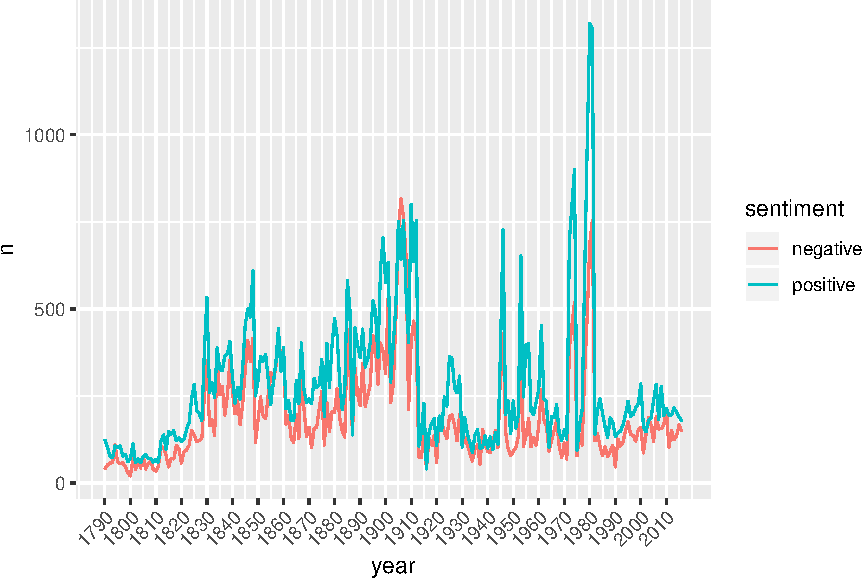
\includegraphics{R-text-analysis_files/figure-latex/sentiment-plot-1.pdf}

TODO: length over time\ldots other similar measures ?
TODO: variation between the different presidents?\\
TODO: topic modeling ?

\bibliography{book.bib,packages.bib}


\end{document}
